\documentclass{beamer}
\usetheme{Madrid}
\usecolortheme{default}
\usepackage{tikz}
\usepackage{amsmath}
\usepackage{booktabs}

\title{Evolutionary Thinking}
\subtitle{A Powerful Lens for Understanding Change}
\author{Brendan Shea, PhD}
\date{Intro to Logic}

\begin{document}
	
	\frame{\titlepage}
	
	% Slide 1: Evolutionary Thinking: A Powerful Lens for Understanding Change
	\begin{frame}
		\frametitle{Evolutionary Thinking: A Powerful Lens for Understanding Change}
		\begin{itemize}
			\item \textbf{Evolutionary thinking} is a way of understanding how things change over time through variation and selection.
			\item This approach began in biology but has spread to many other fields like computer science, economics, and psychology.
			\item Today we'll explore both the power and the limitations of applying evolutionary models to different domains.
			\item By the end, you'll understand when evolutionary thinking helps us explain phenomena and when it can lead us astray.
		\end{itemize}
		\begin{alertblock}{Key Question}
			How can a theory about biological change help us understand everything from computer algorithms to internet memes?
		\end{alertblock}
	\end{frame}
	
	% Slide 2: Charles Darwin: The Revolutionary Naturalist
	\begin{frame}
		\frametitle{Charles Darwin: The Revolutionary Naturalist}
		\begin{itemize}
			\item Charles Darwin (1809-1882) was a British naturalist who fundamentally changed how we understand life on Earth.
			\item His theory of \textbf{evolution by natural selection} provided a scientific explanation for the diversity and complexity of life.
			\item Darwin spent over 20 years gathering evidence before publishing "On the Origin of Species" in 1859.
			\item His ideas were revolutionary because they explained design in nature without requiring a designer.
		\end{itemize}
		\begin{block}{Historical Context}
			Before Darwin, most people believed species were fixed and unchanging. Darwin showed that all life shares common ancestors and changes over time.
		\end{block}
	\end{frame}
	
	% Slide 3: The Voyage of the Beagle: Observations That Changed Science
	\begin{frame}
		\frametitle{The Voyage of the Beagle: Observations That Changed Science}
		\begin{itemize}
			\item From 1831-1836, Darwin sailed around the world as the ship's naturalist on HMS Beagle.
			\item He observed that similar species on different islands had distinct variations suited to their specific environments.
			\item The \textbf{Galápagos finches} showed different beak shapes that matched their food sources: thick beaks for seeds, thin beaks for insects.
			\item These observations suggested that species could change over time to fit their environments.
		\end{itemize}
		\begin{example}
			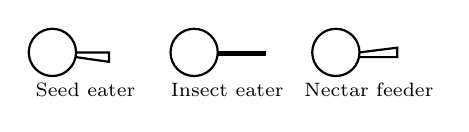
\begin{tikzpicture}[scale=0.6]
				\scriptsize
				% Draw three simple finch heads with different beaks
				\draw[thick] (0,0) circle (0.5cm);
				\draw[thick] (0.5,0) -- (1.2,0) -- (1.2,-0.2) -- (0.5,-0.1);
				\node at (0.7,-0.8) {Seed eater};
				
				\draw[thick] (3,0) circle (0.5cm);
				\draw[thick] (3.5,0) -- (4.5,0) -- (4.5,-0.05) -- (3.5,-0.05);
				\node at (3.7,-0.8) {Insect eater};
				
				\draw[thick] (6,0) circle (0.5cm);
				\draw[thick] (6.5,0) -- (7.3,0.1) -- (7.3,-0.1) -- (6.5,-0.1);
				\node at (6.7,-0.8) {Nectar feeder};
			\end{tikzpicture}
		\end{example}
	\end{frame}
	
	% Slide 4: Natural Selection: The Engine of Evolution
	\begin{frame}
		\frametitle{Natural Selection: The Engine of Evolution}
		\begin{itemize}
			\item \textbf{Natural selection} is the process where organisms with traits better suited to their environment tend to survive and reproduce more.
			\item Darwin identified three requirements for natural selection: variation, inheritance, and differential reproduction.
			\item Over many generations, beneficial traits become more common in a population while harmful traits become rare.
			\item This process is not random—it's directed by the environment and which traits help organisms survive and reproduce.
		\end{itemize}
		\begin{alertblock}{Common Misconception}
			Evolution is NOT about "survival of the fittest" in terms of strength. "Fitness" in evolution means reproductive success—having more offspring that survive.
		\end{alertblock}
	\end{frame}
	
	% Slide 5: Variation, Inheritance, and Differential Survival
	\begin{frame}
		\frametitle{Variation, Inheritance, and Differential Survival}
		\begin{itemize}
			\item \textbf{Variation} means individuals in a population differ in their traits—no two organisms are exactly alike.
			\item \textbf{Inheritance} ensures that offspring resemble their parents more than random individuals in the population.
			\item \textbf{Differential survival and reproduction} occurs when some variants leave more offspring than others.
			\item These three components work together: variation provides options, inheritance preserves successful traits, and differential survival determines which traits spread.
		\end{itemize}
		\begin{block}{The Recipe for Evolution}
			\begin{enumerate}
				\item Individuals vary in their traits
				\item Traits are passed from parents to offspring
				\item Some traits help individuals survive and reproduce better
				\item Result: Populations change over time
			\end{enumerate}
		\end{block}
	\end{frame}
	
	% Slide 6: The Tree of Life: Common Descent
	\begin{frame}
		\frametitle{The Tree of Life: Common Descent}
		\begin{itemize}
			\item \textbf{Common descent} is the idea that all living things share ancestors if we go back far enough in time.
			\item Darwin proposed that life forms a branching tree, with species splitting into new species over millions of years.
			\item This explains why organisms share similar features: they inherited them from common ancestors.
			\item The more recently two species shared an ancestor, the more similar they tend to be.
		\end{itemize}
		\begin{example}
			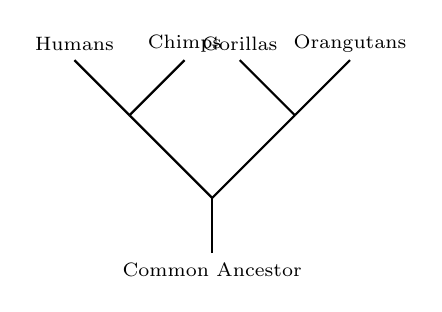
\begin{tikzpicture}[scale=0.7]
				\scriptsize
				% Simple tree diagram
				\draw[thick] (0,0) -- (0,1);
				\draw[thick] (0,1) -- (-1.5,2.5);
				\draw[thick] (0,1) -- (1.5,2.5);
				\draw[thick] (-1.5,2.5) -- (-2.5,3.5);
				\draw[thick] (-1.5,2.5) -- (-0.5,3.5);
				\draw[thick] (1.5,2.5) -- (0.5,3.5);
				\draw[thick] (1.5,2.5) -- (2.5,3.5);
				\node at (-2.5,3.8) {Humans};
				\node at (-0.5,3.8) {Chimps};
				\node at (0.5,3.8) {Gorillas};
				\node at (2.5,3.8) {Orangutans};
				\node at (0,-0.3) {Common Ancestor};
			\end{tikzpicture}
		\end{example}
	\end{frame}
	
	% Slide 7: Evidence for Evolution: Fossils, Anatomy, and Geography
	\begin{frame}
		\frametitle{Evidence for Evolution: Fossils, Anatomy, and Geography}
		\begin{itemize}
			\item \textbf{Fossil evidence} shows how organisms have changed over time, with older fossils generally being simpler and newer ones more complex.
			\item \textbf{Comparative anatomy} reveals similar bone structures in different animals, suggesting they evolved from common ancestors.
			\item \textbf{Biogeography} shows that species distributions make sense based on evolution and continental drift, not random placement.
			\item Multiple independent lines of evidence all point to the same conclusion: species evolve over time.
		\end{itemize}
		\begin{table}
			\centering
			\begin{tabular}{|l|l|}
				\hline
				\textbf{Type of Evidence} & \textbf{Example} \\
				\hline
				Fossils & Whale ancestors with legs \\
				Anatomy & Same bones in human hands and bat wings \\
				Geography & Unique species on isolated islands \\
				DNA & Genetic similarities match predicted relationships \\
				\hline
			\end{tabular}
		\end{table}
	\end{frame}
	
	% Slide 8: Evolution vs. "Just a Theory": Understanding Scientific Theories
	\begin{frame}
		\frametitle{Evolution vs. "Just a Theory": Understanding Scientific Theories}
		\begin{itemize}
			\item In everyday language, "theory" means a guess, but in science, a \textbf{theory} is a well-supported explanation for natural phenomena.
			\item Scientific theories like evolution, gravity, and germ theory are supported by vast amounts of evidence from multiple sources.
			\item Evolution is both a fact (species change over time) and a theory (natural selection explains how).
			\item Theories in science are actually stronger than facts because they explain why things happen, not just that they happen.
		\end{itemize}
		\begin{alertblock}{Important Distinction}
			Scientific theories are not "promoted" to facts when proven. Theories and facts are different things: facts are observations, theories explain those observations.
		\end{alertblock}
	\end{frame}
	
	% Slide 9: Antibiotic Resistance: Evolution in Real Time
	\begin{frame}
		\frametitle{Antibiotic Resistance: Evolution in Real Time}
		\begin{itemize}
			\item \textbf{Antibiotic resistance} occurs when bacteria evolve to survive drugs that once killed them.
			\item When we use antibiotics, most bacteria die, but a few with resistance genes survive and multiply.
			\item These resistant bacteria pass their genes to offspring, creating populations that antibiotics can't kill.
			\item This is evolution by natural selection happening fast enough for us to observe directly in hospitals and labs.
		\end{itemize}
		\begin{alertblock}{Why This Matters}
			Antibiotic resistance causes over 700,000 deaths annually worldwide. Understanding evolution helps doctors use antibiotics more wisely to slow resistance.
		\end{alertblock}
	\end{frame}
	
	% Slide 10: Why Do We Get Wisdom Teeth? Vestigial Structures Explained
	\begin{frame}
		\frametitle{Why Do We Get Wisdom Teeth? Vestigial Structures Explained}
		\begin{itemize}
			\item \textbf{Vestigial structures} are body parts that have lost most or all of their original function through evolution.
			\item Wisdom teeth made sense when our ancestors had larger jaws and needed extra molars to grind tough plant foods.
			\item As human brains evolved to be larger, our jaws became smaller, leaving insufficient room for these teeth.
			\item Other vestigial structures include the appendix, tailbone, and muscles that would move our ears if they still worked.
		\end{itemize}
		\begin{example}
			\scriptsize
			\textbf{Human Vestigial Structures:}
			\begin{itemize}
				\item Wisdom teeth - for grinding plant material
				\item Appendix - possibly for digesting cellulose
				\item Goosebumps - for making fur stand up
				\item Tailbone - remnant of ancestral tail
			\end{itemize}
		\end{example}
	\end{frame}
	
	% Slide 11: The Peacock's Tail: Sexual Selection and Costly Displays
	\begin{frame}
		\frametitle{The Peacock's Tail: Sexual Selection and Costly Displays}
		\begin{itemize}
			\item \textbf{Sexual selection} is evolution driven by competition for mates rather than just survival.
			\item A peacock's elaborate tail actually makes it harder to escape predators, seeming to contradict natural selection.
			\item However, peahens prefer males with impressive tails, so genes for elaborate tails get passed on despite survival costs.
			\item This demonstrates that evolution optimizes for reproductive success, not just survival—sometimes these goals conflict.
		\end{itemize}
		\begin{block}{The Handicap Principle}
			Costly displays can be honest signals of genetic quality. Only healthy peacocks can afford to carry such elaborate, burdensome tails and still survive.
		\end{block}
	\end{frame}
	
	% Slide 12: Convergent Evolution: Why Dolphins and Sharks Look Similar
	\begin{frame}
		\frametitle{Convergent Evolution: Why Dolphins and Sharks Look Similar}
		\begin{itemize}
			\item \textbf{Convergent evolution} occurs when unrelated species independently evolve similar traits in response to similar environments.
			\item Dolphins (mammals) and sharks (fish) both evolved streamlined bodies, fins, and tails for swimming, despite having very different ancestors.
			\item This shows that evolution is not random—similar environmental challenges often produce similar solutions.
			\item Other examples include wings in birds, bats, and insects, or camera eyes in vertebrates and octopuses.
		\end{itemize}
		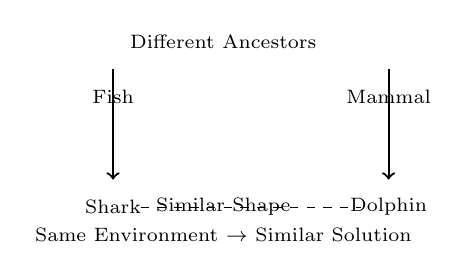
\begin{tikzpicture}[scale=0.7]
			\scriptsize
			% Simple diagram showing convergent evolution
			\node at (0,3) {Different Ancestors};
			\draw[thick,->] (-2,2.5) -- (-2,0.5);
			\draw[thick,->] (3,2.5) -- (3,0.5);
			\node at (-2,0) {Shark};
			\node at (3,0) {Dolphin};
			\node at (-2,2) {Fish};
			\node at (3,2) {Mammal};
			\node at (0,0) {Similar Shape};
			\draw[dashed] (-1.5,0) -- (2.5,0);
			\node at (0,-0.5) {Same Environment $\rightarrow$ Similar Solution};
		\end{tikzpicture}
	\end{frame}
	
	% Slide 13: Coevolution: The Arms Race Between Predators and Prey
	\begin{frame}
		\frametitle{Coevolution: The Arms Race Between Predators and Prey}
		\begin{itemize}
			\item \textbf{Coevolution} occurs when two or more species influence each other's evolution through their interactions.
			\item Predators evolve better hunting abilities, which creates pressure for prey to evolve better defenses, creating an endless cycle.
			\item Cheetahs and gazelles demonstrate this: as cheetahs evolved greater speed, gazelles evolved to run faster and change direction more quickly.
			\item This "evolutionary arms race" explains why both predators and prey often have such remarkable abilities.
		\end{itemize}
		\begin{example}
			\textbf{Coevolution Examples:}
			\begin{tabular}{ll}
				Predator Adaptation & Prey Counter-Adaptation \\
				\hline
				Snake venom toxicity $\uparrow$ & Prey venom resistance $\uparrow$ \\
				Bat echolocation & Moth jamming signals \\
				Spider web strength & Insect escape behaviors \\
			\end{tabular}
		\end{example}
	\end{frame}
	
	% Slide 14: Island Biogeography: Why Island Species Are Unique
	\begin{frame}
		\frametitle{Island Biogeography: Why Island Species Are Unique}
		\begin{itemize}
			\item \textbf{Island biogeography} studies how isolation and limited resources drive unique evolutionary paths on islands.
			\item Island species often evolve from a few founding individuals, leading to rapid diversification to fill empty ecological niches.
			\item Without large predators, some island birds like the dodo lost the ability to fly because flight was no longer necessary for survival.
			\item Islands act as natural laboratories for evolution, showing how geographic isolation leads to new species formation.
		\end{itemize}
		\begin{block}{The Founder Effect}
			When a small group colonizes an island, they carry only a fraction of the genetic variation from the original population. This limited gene pool, combined with new environmental pressures, accelerates evolutionary change.
		\end{block}
	\end{frame}
	
	% Slide 15: Ring Species: Evolution Caught in the Act
	\begin{frame}
		\frametitle{Ring Species: Evolution Caught in the Act}
		\begin{itemize}
			\item \textbf{Ring species} are populations that can interbreed with adjacent populations but not with distant ones, forming a ring of related populations.
			\item California salamanders form a ring around the Central Valley: neighboring populations can mate, but populations at the ends cannot.
			\item This shows us speciation in progress—we can see the gradual changes that eventually prevent interbreeding.
			\item Ring species demonstrate that the boundary between species is not always clear-cut, supporting Darwin's view of gradual change.
		\end{itemize}
		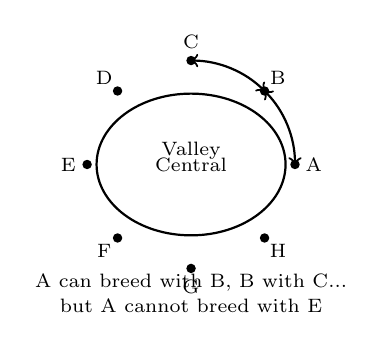
\begin{tikzpicture}[scale=0.6]
			\scriptsize
			% Ring species diagram
			\draw[thick] (0,0) ellipse (2cm and 1.5cm);
			\node at (0,0) {Central};
			\node at (0,0.3) {Valley};
			% Populations around the ring
			\foreach \angle/\name in {0/A, 45/B, 90/C, 135/D, 180/E, 225/F, 270/G, 315/H} {
				\fill (\angle:2.2cm) circle (0.1cm);
				\node at (\angle:2.6cm) {\name};
			}
			% Arrows showing gene flow
			\draw[<->, thick] (0:2.2cm) arc (0:45:2.2cm);
			\draw[<->, thick] (45:2.2cm) arc (45:90:2.2cm);
			\node at (0,-2.5) {A can breed with B, B with C...};
			\node at (0,-3) {but A cannot breed with E};
		\end{tikzpicture}
	\end{frame}
	
	% Slide 16: Evolutionary Development: How Small Changes Make Big Differences
	\begin{frame}
		\frametitle{Evolutionary Development: How Small Changes Make Big Differences}
		\begin{itemize}
			\item \textbf{Evolutionary developmental biology (evo-devo)} studies how changes in developmental genes can produce major evolutionary changes.
			\item Small mutations in "master control genes" can dramatically alter body plans, like changing where legs or wings develop.
			\item The same toolkit of genes controls development across vastly different animals, from flies to humans.
			\item This explains how evolution can produce new body forms relatively quickly through tweaks to developmental timing and patterns.
		\end{itemize}
		\begin{alertblock}{Key Insight}
			Evolution doesn't need to reinvent complex structures from scratch. By changing when and where existing genes are activated during development, evolution can create dramatic new forms from old blueprints.
		\end{alertblock}
	\end{frame}
	
	% Slide 17: Beyond Biology: Can Evolution Explain Other Systems?
	\begin{frame}
		\frametitle{Beyond Biology: Can Evolution Explain Other Systems?}
		\begin{itemize}
			\item Evolutionary thinking can be applied to any system that has variation, selection, and inheritance of traits.
			\item \textbf{Universal Darwinism} is the idea that evolutionary principles work beyond biology in fields like technology, culture, and ideas.
			\item For evolution to work in a domain, we need "things" that can replicate with variation and face selection pressure.
			\item We'll explore how this framework helps us understand changes in technology, economics, and culture—but also where it breaks down.
		\end{itemize}
		\begin{block}{The Universal Algorithm}
			\begin{enumerate}
				\item Create variations of existing solutions
				\item Test which variations perform better
				\item Copy successful variations
				\item Repeat the process
			\end{enumerate}
		\end{block}
	\end{frame}
	
	% Slide 18: Evolutionary Computation: Teaching Computers to Evolve Solutions
	\begin{frame}
		\frametitle{Evolutionary Computation: Teaching Computers to Evolve Solutions}
		\begin{itemize}
			\item \textbf{Evolutionary algorithms} use principles of natural selection to solve complex problems that are hard to solve directly.
			\item Programmers create a population of random solutions, test them, keep the best ones, and "breed" them with mutations.
			\item After many generations, the algorithm evolves solutions that no human programmer directly designed.
			\item This approach has solved problems in engineering, scheduling, and design that were too complex for traditional methods.
		\end{itemize}
		\begin{example}
			\textbf{Steps in a Genetic Algorithm:}
			\scriptsize
			\begin{enumerate}
				\item Generate 100 random solutions
				\item Score each solution's performance
				\item Select the top 20 performers
				\item Create 100 new solutions by combining and mutating the winners
				\item Repeat until solution is good enough
			\end{enumerate}
		\end{example}
	\end{frame}
	
	% Slide 19: Case Study: NASA's Evolved Antenna Design
	\begin{frame}
		\frametitle{Case Study: NASA's Evolved Antenna Design}
		\begin{itemize}
			\item NASA needed a small, efficient antenna for a spacecraft but traditional designs weren't meeting all requirements.
			\item Engineers used evolutionary algorithms to "evolve" antenna shapes, starting with random wire configurations.
			\item The algorithm tested each design in simulation, keeping designs with better signal properties and discarding poor performers.
			\item The final evolved antenna looked bizarre—like bent paperclips—but outperformed human-designed antennas.
		\end{itemize}
		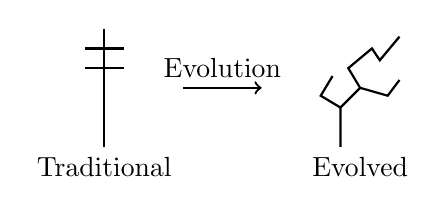
\begin{tikzpicture}[scale=0.5]
			% Traditional antenna (left)
			\draw[thick] (-5,0) -- (-5,3);
			\draw[thick] (-5.5,2.5) -- (-4.5,2.5);
			\draw[thick] (-5.5,2) -- (-4.5,2);
			\node at (-5,-0.5) {Traditional};
			
			% Arrow
			\draw[thick,->] (-3,1.5) -- (-1,1.5);
			\node at (-2,2) {Evolution};
			
			% Evolved antenna (right) - irregular shape
			\draw[thick] (1,0) -- (1,1) -- (1.5,1.5) -- (1.2,2) -- (1.8,2.5) -- (2,2.2) -- (2.5,2.8);
			\draw[thick] (1,1) -- (0.5,1.3) -- (0.8,1.8);
			\draw[thick] (1.5,1.5) -- (2.2,1.3) -- (2.5,1.7);
			\node at (1.5,-0.5) {Evolved};
		\end{tikzpicture}
	\end{frame}
	
	% Slide 20: Memetics: Can Ideas Evolve Like Organisms?
	\begin{frame}
		\frametitle{Memetics: Can Ideas Evolve Like Organisms?}
		\begin{itemize}
			\item \textbf{Memes} (in the original sense) are units of cultural information that spread from person to person, like genes spread biologically.
			\item Richard Dawkins proposed that ideas, behaviors, and cultural practices evolve through variation, selection, and transmission.
			\item Successful memes spread because they are memorable, useful, or emotionally compelling—not necessarily because they're true.
			\item This framework helps explain how rumors, fashions, and beliefs spread and change through populations over time.
		\end{itemize}
		\begin{alertblock}{Important Caveat}
			Unlike genes, memes can be intentionally modified, spread horizontally between unrelated people, and combine in complex ways. This makes memetic evolution less predictable than biological evolution.
		\end{alertblock}
	\end{frame}
	
	% Slide 21: Internet Memes: Natural Selection in Digital Culture
	\begin{frame}
		\frametitle{Internet Memes: Natural Selection in Digital Culture}
		\begin{itemize}
			\item Internet memes demonstrate evolution in real-time: images and jokes mutate as people modify them, and only the funniest or most relatable versions spread.
			\item \textbf{Variation} occurs when users edit memes with new text, images, or contexts to create slightly different versions.
			\item \textbf{Selection} happens through likes, shares, and reposts—engaging content survives while boring content disappears.
			\item Memes evolve to fit their "environment" (different social media platforms) with different formats succeeding on Twitter versus TikTok.
		\end{itemize}
		\begin{example}
			\scriptsize
			\textbf{Meme Evolution Timeline:}
			\begin{itemize}
				\item Original: Simple image with text
				\item Mutation 1: New caption for different context
				\item Mutation 2: Combined with another meme format
				\item Result: Hybrid meme that spreads faster than either parent
			\end{itemize}
		\end{example}
	\end{frame}
	
	% Slide 22: Evolutionary Economics: Markets as Ecosystems
	\begin{frame}
		\frametitle{Evolutionary Economics: Markets as Ecosystems}
		\begin{itemize}
			\item \textbf{Evolutionary economics} treats businesses like organisms competing for resources (customers and capital) in market ecosystems.
			\item Companies with profitable strategies survive and expand, while those with poor strategies go bankrupt and disappear.
			\item Business practices spread through imitation—successful strategies are copied by competitors, like beneficial genes spreading through populations.
			\item Markets create selection pressure: consumer preferences, regulations, and competition determine which business "traits" succeed.
		\end{itemize}
		\begin{block}{Economic Natural Selection}
			Just as predators select for faster prey, economic competition selects for more efficient companies. Inefficient businesses are "eaten" by competitors or starve from lack of customers.
		\end{block}
	\end{frame}
	
	% Slide 23: Case Study: The Rise and Fall of Blockbuster vs. Netflix
	\begin{frame}
		\frametitle{Case Study: The Rise and Fall of Blockbuster vs. Netflix}
		\begin{itemize}
			\item Blockbuster dominated video rental with 9,000 stores, perfectly adapted to the 1990s "environment" of physical media and browsing.
			\item Netflix began as a "mutation"—DVDs by mail—which seemed inferior but avoided late fees and store visits.
			\item When the environment changed (internet speeds increased), Netflix evolved streaming while Blockbuster couldn't adapt quickly enough.
			\item This demonstrates economic extinction: Blockbuster was too specialized for its niche and couldn't evolve when conditions changed.
		\end{itemize}
		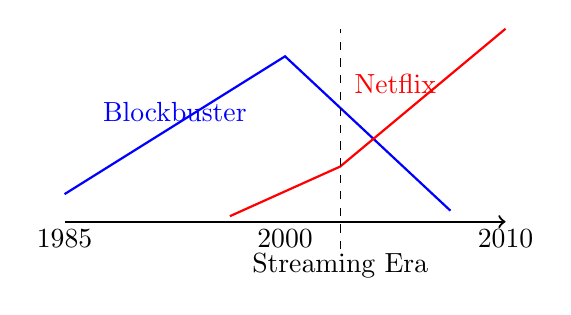
\begin{tikzpicture}[scale=0.7]
			% Timeline
			\draw[thick,->] (0,0) -- (8,0);
			\node at (0,-0.3) {1985};
			\node at (4,-0.3) {2000};
			\node at (8,-0.3) {2010};
			% Blockbuster line
			\draw[thick,blue] (0,0.5) -- (4,3) -- (7,0.2);
			\node[blue] at (2,2) {Blockbuster};
			% Netflix line
			\draw[thick,red] (3,0.1) -- (5,1) -- (8,3.5);
			\node[red] at (6,2.5) {Netflix};
			% Environment change
			\draw[dashed] (5,-0.5) -- (5,3.5);
			\node at (5,-0.8) {Streaming Era};
		\end{tikzpicture}
	\end{frame}
	
	% Slide 24: Evolutionary Game Theory: Cooperation and Competition
	\begin{frame}
		\frametitle{Evolutionary Game Theory: Cooperation and Competition}
		\begin{itemize}
			\item \textbf{Evolutionary game theory} studies how strategies for interaction evolve in populations over time.
			\item Unlike traditional game theory, players don't choose strategies rationally—successful strategies spread through the population.
			\item This explains how cooperation can evolve even among selfish individuals if it provides mutual benefits over time.
			\item Different strategies (like "always cooperate" or "tit-for-tat") compete, with successful ones becoming more common.
		\end{itemize}
		\begin{table}
			\centering
			\small
			\begin{tabular}{|l|c|c|}
				\hline
				\textbf{Strategy} & \textbf{Short-term} & \textbf{Long-term} \\
				\hline
				Always Defect & Wins initially & Dies out \\
				Always Cooperate & Exploited & Dies out \\
				Tit-for-Tat & Moderate & Dominates \\
				\hline
			\end{tabular}
			\caption{Evolution of strategies in repeated interactions}
		\end{table}
	\end{frame}
	
	% Slide 25: The Prisoner's Dilemma: Why Cooperation Evolves
	\begin{frame}
		\frametitle{The Prisoner's Dilemma: Why Cooperation Evolves}
		\begin{itemize}
			\item The \textbf{Prisoner's Dilemma} shows why cooperation is difficult: betraying your partner gives a better outcome regardless of what they do.
			\item In single interactions, defection dominates, but in repeated interactions, cooperative strategies can evolve and spread.
			\item "Tit-for-tat" (cooperate first, then copy opponent's last move) evolves because it rewards cooperation and punishes defection.
			\item This explains real-world cooperation: from cleaner fish and their hosts to international trade agreements that build on repeated interactions.
		\end{itemize}
		\begin{example}
			\begin{tabular}{|c|c|c|}
				\hline
				& \textbf{Cooperate} & \textbf{Defect} \\
				\hline
				\textbf{Cooperate} & Both get 3 & You get 0, they get 5 \\
				\hline
				\textbf{Defect} & You get 5, they get 0 & Both get 1 \\
				\hline
			\end{tabular}
			\\[0.3cm]
			Mutual cooperation (3,3) beats mutual defection (1,1), but defection tempts!
		\end{example}
	\end{frame}
	
	% Slide 26: Cultural Evolution: How Human Societies Change Over Time
	\begin{frame}
		\frametitle{Cultural Evolution: How Human Societies Change Over Time}
		\begin{itemize}
			\item \textbf{Cultural evolution} applies evolutionary thinking to understand how languages, religions, technologies, and customs change over time.
			\item Unlike genetic evolution, cultural traits spread horizontally (between peers) and can change within a single generation.
			\item Successful cultural practices spread through teaching, imitation, and social pressure rather than biological reproduction.
			\item This explains phenomena like why some languages dominate while others go extinct, or how technologies spread through societies.
		\end{itemize}
		\begin{block}{Key Differences from Biological Evolution}
			\begin{itemize}
				\item Speed: Cultural evolution can happen in years, not millennia
				\item Direction: Humans can intentionally guide cultural change
				\item Inheritance: We can "inherit" traits from many cultural "parents"
			\end{itemize}
		\end{block}
	\end{frame}
	
	% Slide 27: When Evolutionary Thinking Goes Wrong
	\begin{frame}
		\frametitle{When Evolutionary Thinking Goes Wrong}
		\begin{itemize}
			\item Evolutionary thinking is powerful, but applying it carelessly to human society has led to harmful ideologies and bad science.
			\item \textbf{Social Darwinism} wrongly used evolution to justify inequality, claiming the poor deserved their fate due to "inferior fitness."
			\item Some evolutionary psychology makes untestable "just-so stories" that claim to explain modern behavior through prehistoric scenarios.
			\item These misuses remind us that descriptive science (what is) should not determine prescriptive ethics (what ought to be).
		\end{itemize}
		\begin{alertblock}{Critical Thinking Required}
			When someone uses evolutionary arguments about human society, ask: Is this testable? Are there alternative explanations? Are they confusing "is" with "ought"? Are they oversimplifying complex social phenomena?
		\end{alertblock}
	\end{frame}
	
	% Slide 28: Social Darwinism: The Dangerous Misapplication of Natural Selection
	\begin{frame}
		\frametitle{Social Darwinism: The Dangerous Misapplication of Natural Selection}
		\begin{itemize}
			\item \textbf{Social Darwinism} emerged in the late 1800s, claiming that social inequality reflected natural selection among humans.
			\item Proponents argued the wealthy were "naturally superior" and helping the poor interfered with evolution—a complete misunderstanding of Darwin's ideas.
			\item This pseudoscience was used to justify colonialism, racism, and eugenics programs that caused immense human suffering.
			\item Darwin himself opposed these ideas, noting that human compassion and cooperation were evolved traits that made us successful.
		\end{itemize}
		\begin{example}
			\scriptsize
			\textbf{Flawed Logic of Social Darwinism:}
			\begin{enumerate}
				\item Assumes wealth = biological fitness (false)
				\item Ignores that cooperation is adaptive (false)
				\item Commits naturalistic fallacy (natural $\neq$ good)
				\item Misunderstands "fitness" (reproduction, not strength)
			\end{enumerate}
		\end{example}
	\end{frame}
	
	% Slide 29: Scientific Racism: How Evolution Was Weaponized
	\begin{frame}
		\frametitle{Scientific Racism: How Evolution Was Weaponized}
		\begin{itemize}
			\item \textbf{Scientific racism} misused evolutionary concepts to create false hierarchies among human populations based on supposed "evolutionary advancement."
			\item Racist scientists claimed some races were "more evolved" than others, ignoring that all humans share recent common ancestry.
			\item Modern genetics proves human populations have remarkably little genetic variation—we're one of the least genetically diverse species.
			\item These pseudoscientific ideas caused real harm through discriminatory policies, forced sterilizations, and genocide.
		\end{itemize}
		\begin{alertblock}{The Scientific Reality}
			All human populations have been evolving for exactly the same amount of time since our common ancestors. There is no "more evolved" or "less evolved" when it comes to human groups—evolution doesn't work that way.
		\end{alertblock}
	\end{frame}
	
	% Slide 30: Evolutionary Psychology: Promising Field or "Just-So Stories"?
	\begin{frame}
		\frametitle{Evolutionary Psychology: Promising Field or "Just-So Stories"?}
		\begin{itemize}
			\item \textbf{Evolutionary psychology} attempts to explain human behavior through adaptations to ancestral environments.
			\item Strong claims include universal facial expressions and fear of snakes/spiders—these have good evidence across cultures.
			\item Weak claims make untestable assumptions about prehistoric life to explain modern behaviors like shopping or political preferences.
			\item The field struggles because we can't directly observe prehistoric human behavior or run controlled experiments on human evolution.
		\end{itemize}
		\begin{block}{How to Evaluate Evolutionary Psychology Claims}
			\textbf{Good claims:} Make testable predictions, have cross-cultural evidence, consider alternative explanations, acknowledge limitations\\
			\textbf{Bad claims:} Tell neat stories without evidence, ignore cultural variation, claim single evolutionary causes for complex behaviors
		\end{block}
	\end{frame}
	
	% Slide 31: The Naturalistic Fallacy: Why "Natural" Doesn't Mean "Good"
	\begin{frame}
		\frametitle{The Naturalistic Fallacy: Why "Natural" Doesn't Mean "Good"}
		\begin{itemize}
			\item The \textbf{naturalistic fallacy} is the error of assuming that whatever is "natural" or evolved must be morally good or desirable.
			\item Evolution produces many behaviors we consider immoral: infanticide, rape, and parasitism are all "natural" strategies in some species.
			\item Human morality often requires us to overcome our evolved impulses—cooperation with strangers and universal human rights are cultural inventions.
			\item Understanding the evolutionary origins of behavior can inform but should never determine our ethical choices.
		\end{itemize}
		\begin{example}
			\scriptsize
			\textbf{Natural Does Not Equal Good:}
			\begin{tabular}{|l|l|}
				\hline
				\textbf{Natural but Bad} & \textbf{Unnatural but Good} \\
				\hline
				Disease and parasites & Medicine and vaccines \\
				Tribal warfare & International cooperation \\
				Death in childbirth & Modern healthcare \\
				Might makes right & Equal rights and justice \\
				\hline
			\end{tabular}
		\end{example}
	\end{frame}
	
	% Slide 32: Limits of Evolutionary Thinking: What It Can't Explain
	\begin{frame}
		\frametitle{Limits of Evolutionary Thinking: What It Can't Explain}
		\begin{itemize}
			\item Evolutionary thinking works best when there's true replication with inheritance, variation, and selection over many generations.
			\item It struggles with one-time historical events, conscious design, and systems where "inheritance" is unclear or absent.
			\item Individual creativity, mathematical proofs, and philosophical arguments don't evolve—they're created by conscious minds.
			\item Evolution explains change over time but not necessarily progress, purpose, or the origin of a particular new idea.
		\end{itemize}
		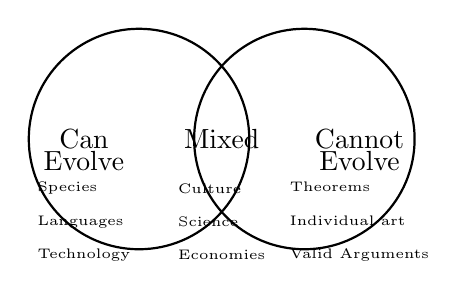
\begin{tikzpicture}[scale=0.7]
			% Venn diagram showing overlap
			\draw[thick] (0,0) circle (2cm);
			\draw[thick] (3,0) circle (2cm);
			\node at (-1,0) {Can};
			\node at (-1,-0.4) {Evolve};
			\node at (4,0) {Cannot};
			\node at (4,-0.4) {Evolve};
			\node at (1.5,0) {Mixed};
			% Examples
			\node[align=left] at (-1,-1.5) {\tiny Species\\\tiny Languages\\\tiny Technology};
			\node[align=left] at (4,-1.5) {\tiny Theorems\\\tiny Individual art\\\tiny Valid Arguments};
			\node[align=left] at (1.5,-1.5) {\tiny Culture\\\tiny Science\\\tiny Economies};
		\end{tikzpicture}
	\end{frame}
	
	% Slide 33: The Power and Peril of Metaphorical Thinking
	\begin{frame}
		\frametitle{The Power and Peril of Metaphorical Thinking}
		\begin{itemize}
			\item Evolutionary thinking is essentially a \textbf{metaphor}—we see patterns from biology and apply them to other domains.
			\item Metaphors can reveal hidden similarities and generate new insights, like seeing markets as ecosystems or ideas as replicators.
			\item However, metaphors can also mislead us when we forget they're simplifications and push them beyond their useful limits.
			\item The key is knowing when evolutionary thinking illuminates a problem and when it obscures important differences.
		\end{itemize}
		\begin{block}{Using Metaphors Wisely}
			\textbf{Good use:} "Companies compete like species" helps us see market dynamics\\
			\textbf{Bad use:} "Poor people are unfit" ignores social structures and human values\\
			\textbf{Key:} Remember what the metaphor highlights AND what it hides
		\end{block}
	\end{frame}
	
	% Slide 34: Good Evolutionary Explanations: Testable, Predictive, and Humble
	\begin{frame}
		\frametitle{Good Evolutionary Explanations: Testable, Predictive, and Humble}
		\begin{itemize}
			\item \textbf{Testable} explanations make specific predictions we can check, not just tell plausible stories about the past.
			\item \textbf{Predictive} power means the explanation helps us anticipate future changes, like predicting antibiotic resistance.
			\item \textbf{Humble} explanations acknowledge uncertainty, consider alternatives, and recognize the limits of the evolutionary framework.
			\item The best evolutionary thinking generates new research questions rather than claiming to have all the answers.
		\end{itemize}
		\begin{example}
			\scriptsize
			\textbf{Comparing Evolutionary Claims:}
			\begin{itemize}
				\item[\checkmark] "Bacteria will evolve resistance to new antibiotics" (testable, predictive)
				\item[\checkmark] "Island species will be vulnerable to invasive predators" (testable, predictive)
				\item[X] "Humans shop because we evolved to gather berries" (untestable story)
				\item[X] "Rich people are evolutionarily superior" (value judgment, not science)
			\end{itemize}
		\end{example}
	\end{frame}
	
	% Slide 35: Evolution as a Tool, Not a Worldview
	\begin{frame}
		\frametitle{Evolution as a Tool, Not a Worldview}
		\begin{itemize}
			\item Evolution is a scientific tool for understanding change in populations over time—nothing more, nothing less.
			\item It doesn't tell us what we should value, how to treat each other, or what makes life meaningful.
			\item Understanding evolution is compatible with diverse worldviews, ethical systems, and personal beliefs about purpose and meaning.
			\item We can use evolutionary insights to solve problems while maintaining our commitment to human dignity, justice, and compassion.
		\end{itemize}
		\begin{alertblock}{Remember}
			Evolution explains how we got here, not where we should go. It describes the process of change, not the purpose of existence. Use it as a powerful tool for understanding, not as a replacement for ethics or meaning.
		\end{alertblock}
	\end{frame}
	
	% Slide 36: Questions for Further Thought: Where Else Might Evolution Apply?
	\begin{frame}
		\frametitle{Questions for Further Thought: Where Else Might Evolution Apply?}
		\begin{itemize}
			\item How might evolutionary thinking help us understand the development of artificial intelligence and machine learning?
			\item Could evolutionary principles explain how art styles, music genres, or fashion trends change over time?
			\item What are the dangers of applying evolutionary thinking to education, politics, or social policy?
			\item Where do you see variation, selection, and inheritance in your own life—and where don't you?
		\end{itemize}
		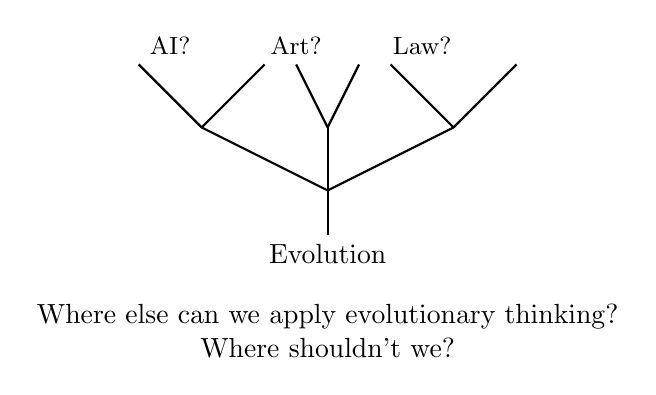
\begin{tikzpicture}[scale=0.8]
			% Thought bubble diagram
			\node at (0,0) {Evolution};
			\draw[thick] (0,0.3) -- (0,1);
			\draw[thick] (0,1) -- (-2,2);
			\draw[thick] (0,1) -- (0,2);
			\draw[thick] (0,1) -- (2,2);
			\draw[thick] (-2,2) -- (-3,3);
			\draw[thick] (-2,2) -- (-1,3);
			\draw[thick] (0,2) -- (-0.5,3);
			\draw[thick] (0,2) -- (0.5,3);
			\draw[thick] (2,2) -- (1,3);
			\draw[thick] (2,2) -- (3,3);
			\node at (-2.5,3.3) {\small AI?};
			\node at (-0.5,3.3) {\small Art?};
			\node at (1.5,3.3) {\small Law?};
			\node at (0,-1) {Where else can we apply evolutionary thinking?};
			\node at (0,-1.5) {Where shouldn't we?};
		\end{tikzpicture}
	\end{frame}
\end{document}